\documentclass[a4paper,11pt]{article}
\usepackage{epsfig}
\usepackage[scaled=0.98]{helvet}
\usepackage{times}
\usepackage{inconsolata}
\usepackage[total={6.25in,8.55in}]{geometry}
\usepackage{fancyhdr}
\pagestyle{fancy}
\usepackage{sectsty}
\usepackage{titlesec}
\usepackage{fancyvrb}
\usepackage{lscape}
\usepackage{color}

\newcommand{\mytitle}{Designing the Crawler}
\newcommand{\theauthor}{Gagarine Yaikhom}
\newcommand{\trid}{{\tt TR-MRCH-DCC-GY012}}

\lhead{MRC Harwell}
\chead{}
\rhead{\small\trid: \mytitle}
\lfoot{Last modified: \today}
\cfoot{}
\rfoot{\thepage}
\renewcommand{\headrulewidth}{0.4pt}
\renewcommand{\footrulewidth}{0.4pt}
\allsectionsfont{\normalsize\sffamily}
\titlelabel{\thetitle.\quad}

\begin{document}

\begin{titlepage}
\centering

\vspace*{3.5cm}

\huge{\mytitle}

\vspace*{1.5cm}

\large{\tt \trid}

\smallskip

\large{\today}

\vspace*{1.5cm}

\large{\theauthor}

\vfill

\begin{abstract}
The {\sl IMPC Data Coordination Centre} provides computational services that simplify the collection, collation, storage, retrieval and analysis of phenotype data. The primary objective of the data upload and quality control interfaces is to provide a consistent and interactive centralised management system for tracking the collection of data from various research centres, and for carrying out quality control over the collected data before they are made available to the general public and to researchers throughout the world. In this report, we discuss the design of the crawler and associated tracking system that is currently deployed at the Data Coordination Centre. This report does not address areas related to the quality control system or the tracker web interface. 
\end{abstract}

\vfill

\vfill


\epsfig{file=assets/WG10-Pantone-Harwell,scale=1}

\end{titlepage}

\section{Introduction}
Phenotyping research produces large quantities of data that must be stored in an efficient and reliable data warehouse. This requires coordination between the various research centres that are producing the data to agree upon a standardisation of the experimental procedures that are used to collect the data. These are referred to as the {\sl Standard Operating Procedures} (SOP) and they provide the experimenter with guidelines on how the experiment should be carried out, and what data must be recorded. The {\sl IMPC Data Coordination Centre} (DCC) here at MRC Harwell uses SOPs specified in the {\sl International Mouse Phenotyping Resource of Standardised Screens}, or IMPReSS for short.

While some of the mechanical factors may be standardised to an acceptable degree, uncontrollable environmental factors specific to a given research institute may skew the data to an unacceptable degree. This prevents the data from being automatically adjusted to make them compatible with the rest of the data from other research centres. To control such variations and to detect data anomaly, human intervention is sometimes necessary to validate the data. This forms the quality control phase, where the data and annotations are examined by the {\sl data wranglers}, and any anomaly is identified and resolved. The DCC provides services that simplify the processes for data upload, tracking and quality control.

\section{Data collection}

\begin{figure}[htbp]
\centering
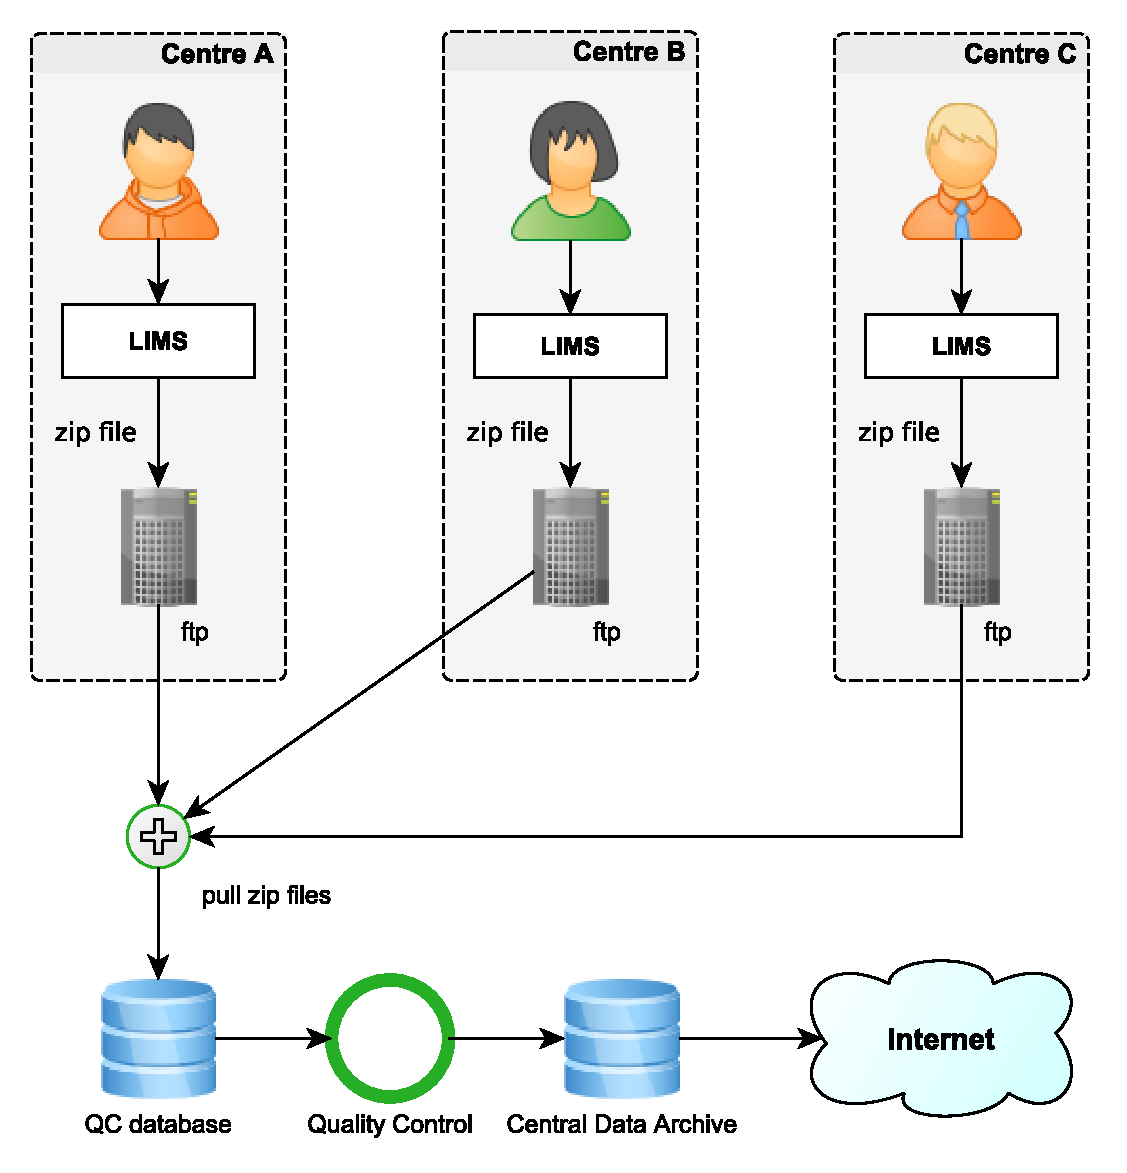
\epsfig{file=assets/pull_arch,scale=0.5}
\caption{Data collection, export, upload, QC and publication.\label{fig:pull architecture}}
\end{figure}

To understand the requirements for the crawler and the tracking system, we must first understand the IMPC workflow which outlines how the data is collected, uploaded, quality controlled, annotated and eventually published to the outside world.

The higher level processes are shown in Figure~\ref{fig:pull architecture}. In this diagram, three centres are collecting and providing experimental data to the DCC. Each of these centres are {\sl not} required to use a specific system for collecting data; each centre is free to choose whichever system is suitable. What matters is that when the centres upload their data to the DCC, their {\sl Laboratory Information Management System} (LIMS) should export the selected data into a standardised format that has been agreed by all of the participating centres and the DCC.

\section{Exporting data from LIMS}

The current data upload process is based on a {\sl pull} architecture. Data from the research centres are not uploaded immediately into the DCC databases. Instead, the data crawlers at the DCC periodically pull the data files from the research centres. This architecture is shown in Figure~\ref{fig:pull architecture}. All of the centres make their data available at specific local ftp/sFtp servers, which are referred to as {\sl file sources}. The DCC crawlers periodically check all of these file sources, and retrieve newly added data files. These files are then downloaded and processed at the DCC. Any issues identified during the processing is tracked and made available through the tracker web interface.

\begin{figure}[htbp]
\centering
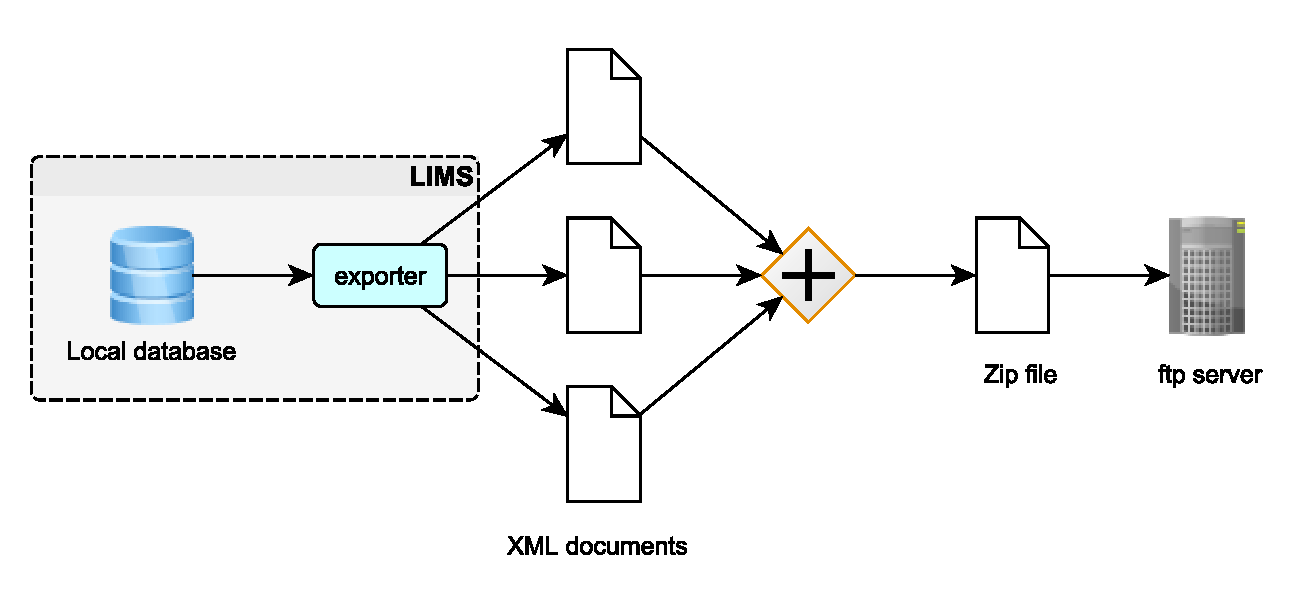
\epsfig{file=assets/exporting,scale=0.5}
\caption{Exporting data to the file sources.\label{fig:exporting to ftp}}
\end{figure}

In the IMPC workflow, after the data has been collected in the local LIMS, they are then exported to the local file source hosted by the centre. To export the data, the LIMS system first generates XML documents that contain the data to be exported. All of these XML documents are then compressed into a zip archive, which is then stored locally in one of the file sources. This is shown in Figure~\ref{fig:exporting to ftp}.

Each of the files generated, both XML documents and zip archives containing them, should adhere to the IMPC file naming convention for it to be processed.

\section{The Crawler architecture}

The crawler uses a multithreaded architecture. Each of the periodic crawling happens inside a crawling session. A session consists of several processing phases. After a session has been initiated, the session thread starts a download manager. The task of the download manager is to spawn multiple threads for each of the file sources (i.e., ftp/sFtp servers) hosted by each of the centres. Each of these threads crawl one of the file sources by visiting the {\tt add}, {\tt delete} and {\tt edit} directories. The directories identify the action to be carried out using the files in those directories. This relationship is shown in Figure~\ref{fig:concept relationship}.

\begin{figure}[htbp]
\centering
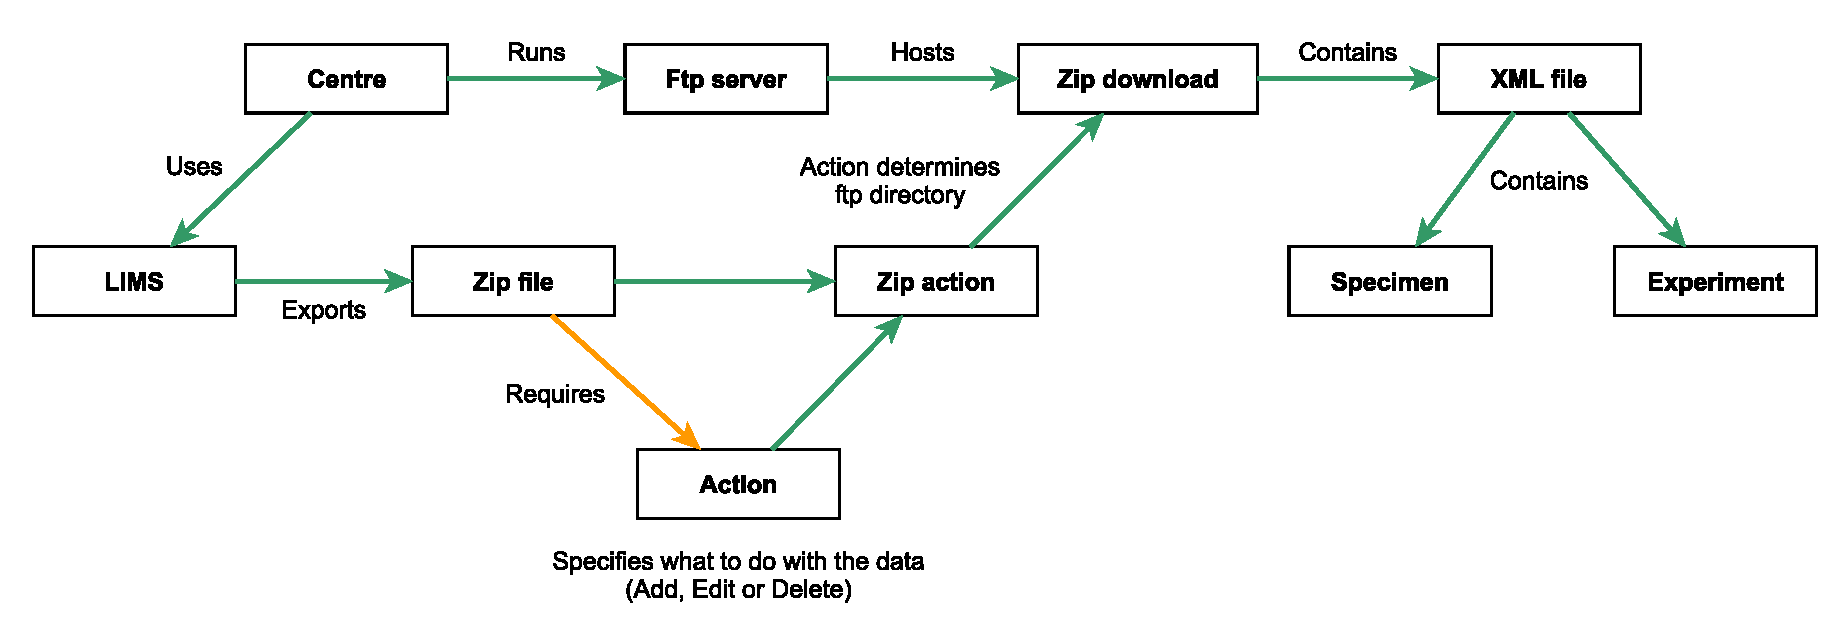
\epsfig{file=assets/concept_relationship,scale=0.5}
\caption{Relationship between concepts.\label{fig:concept relationship}}
\end{figure}

During the crawling, each crawler thread identifies new zip files that have not be processed. When choosing zip files, the crawler ignores files that do not conform to the IMPC file naming convention. For each of the files that should be processed, the crawler makes an entry to the tracker database identifying which file to download from which file source. The file download does not start immediately.

\begin{figure}[htbp]
\centering
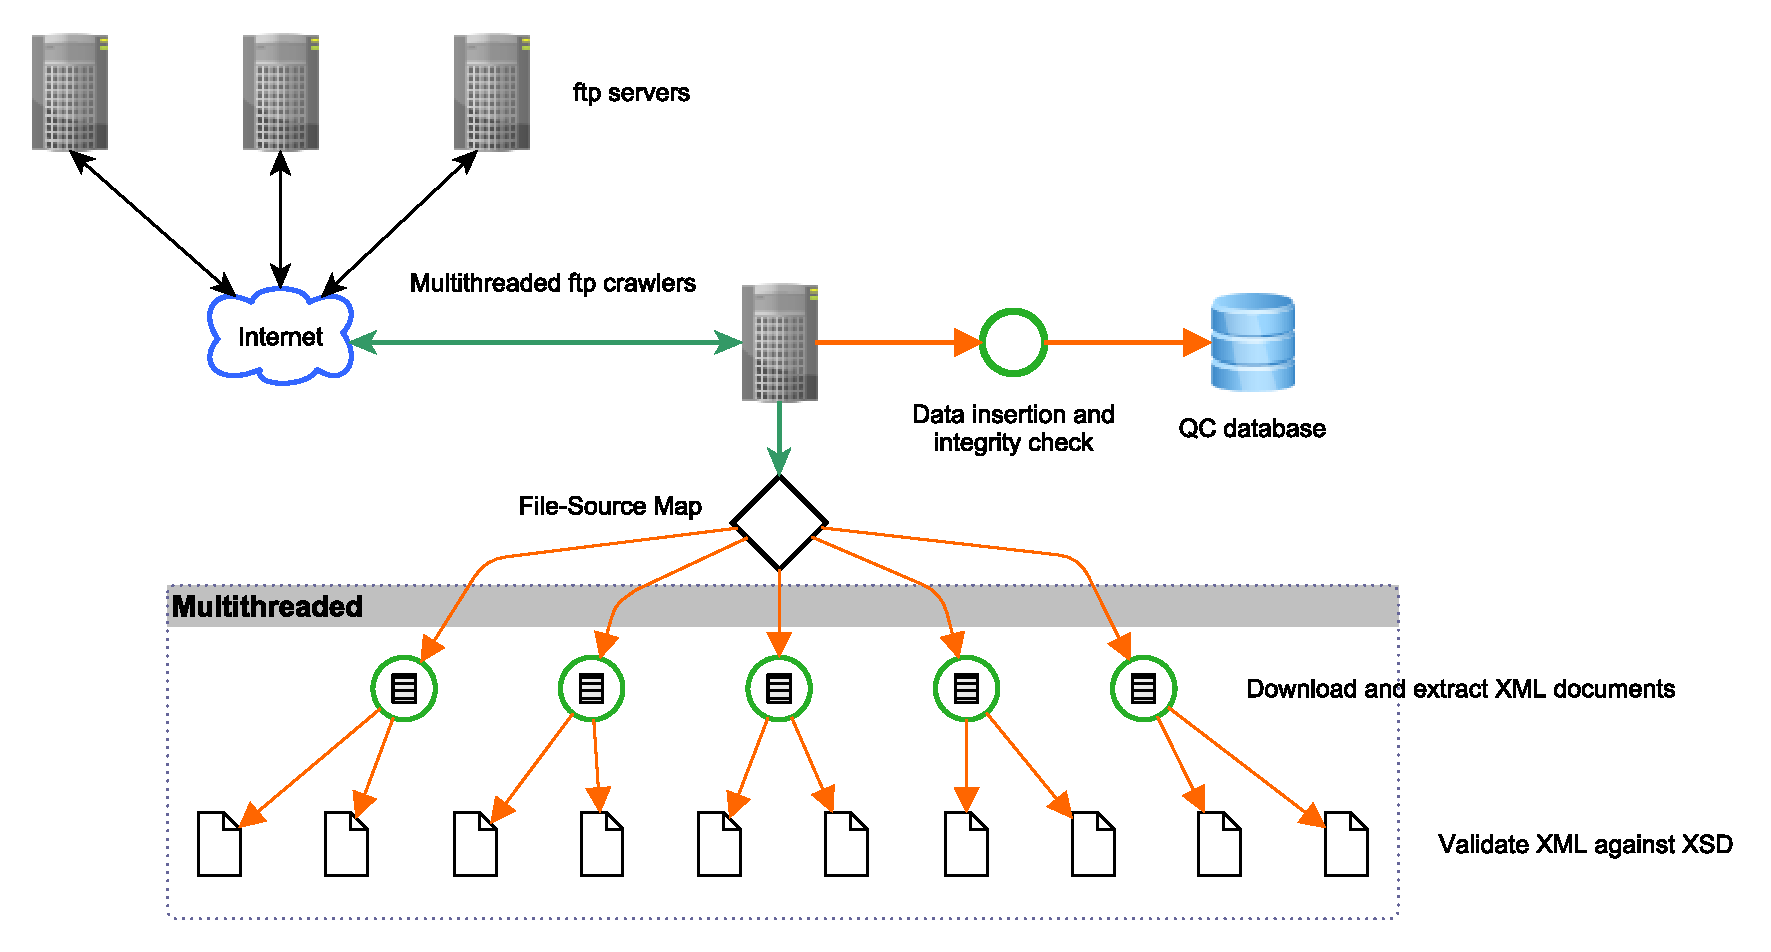
\epsfig{file=assets/crawler_architecture,scale=0.5}
\caption{Crawler architecture.\label{fig:crawler architecture}}
\end{figure}

Once all of the crawling threads have returned, the download manager initiates the download and processing phase. In this phase, the download manager creates a thread pool of downloaders using the size of the thread pool supplied by the user on the command line. The responsibility for each of these threads is to download and process all of the zip files that were mapped out by the crawlers.

Once all of the zip files have been downloaded and processed, the crawler begins the data insertion and data integrity checks. Since there may be implied dependencies between multiple files, the crawler does not multithread the data insertion and data integrity checks. They are carried out sequentially.

\begin{figure}[htbp]
\centering
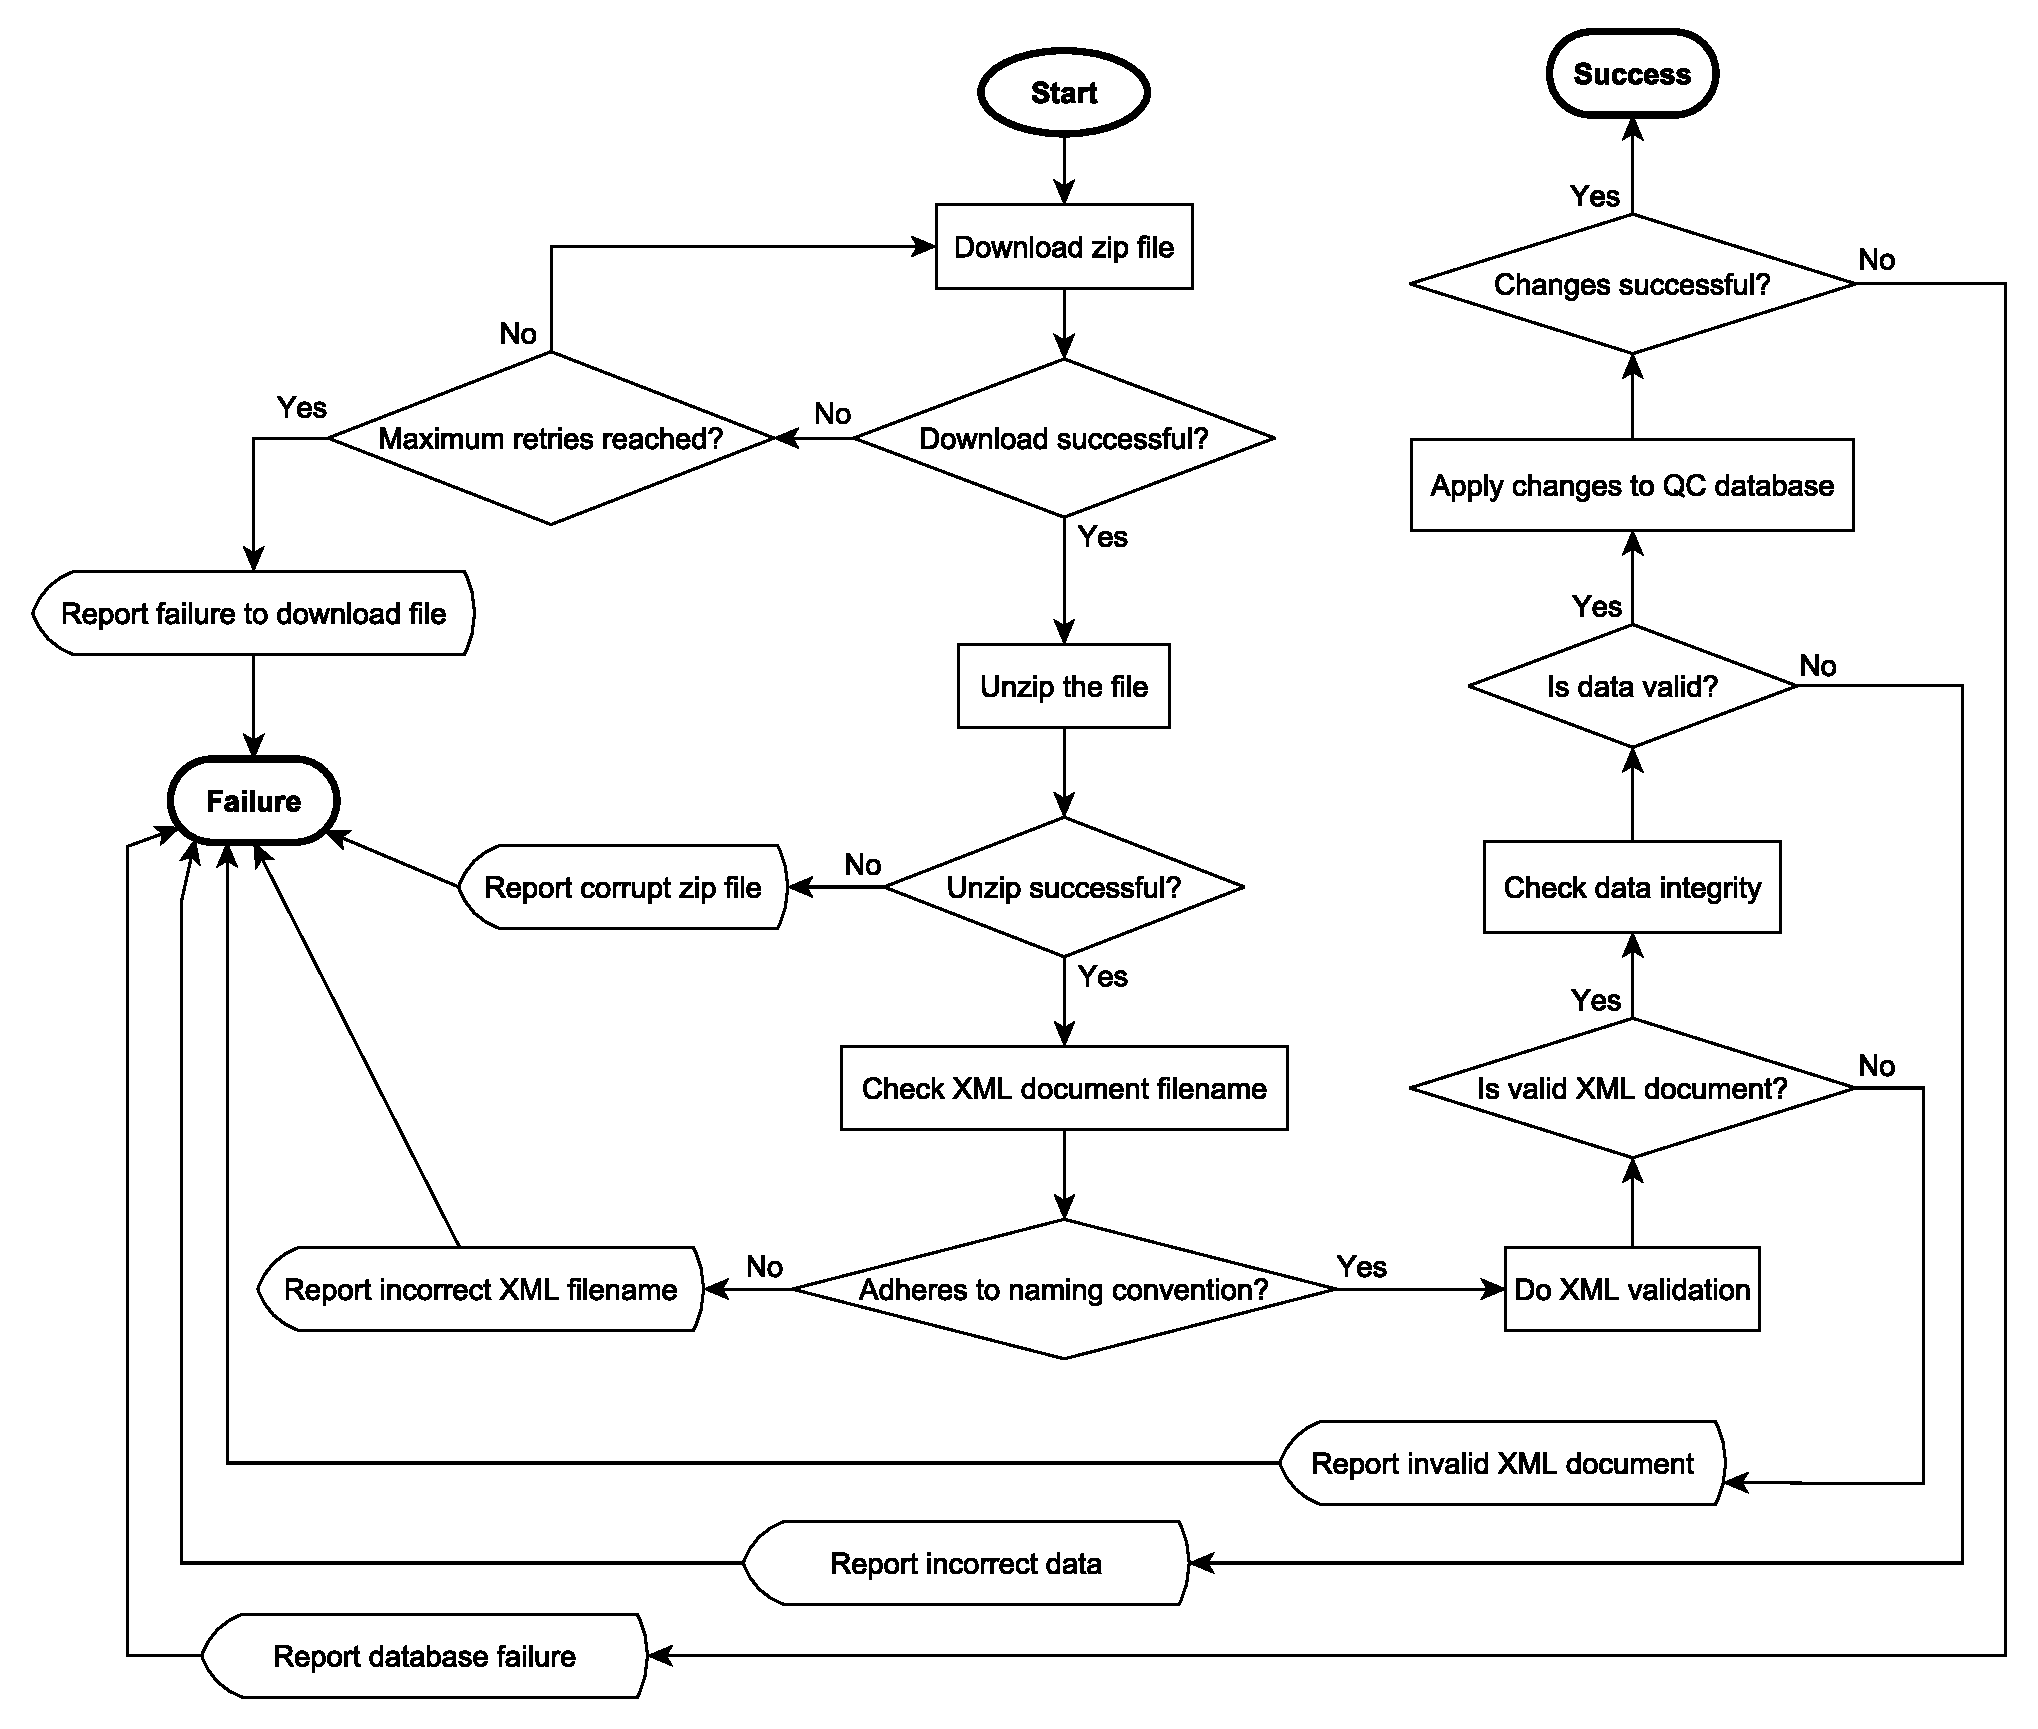
\epsfig{file=assets/processing_flowchart,scale=0.45}
\caption{A flow chart of the processing phases.\label{fig:processing flowchart}}
\end{figure}

After a zip file has been downloaded, the downloader thread extracts the contents of the zip file by creating a directory that is private to the file being extracted. This allows multiple zip files to have contents that share the same file name. If the extraction was successful, the downloader creates a thread pool and spawns multiple processing threads, each thread responsible for validating the structure of the extracted XML document. This validation is carried out using the IMPC data transfer format available as XSD (XML Schema Definition language) schemas. Only files that pass this validation are processed by the data insertion phase.

An overview of the processing phases are shown in Figure~\ref{fig:processing flowchart}.

\begin{landscape}

\section{The tracker database}

The tracker database is named, {\tt phenodcc\_tracker}. The schema is available in the {\tt phenodcc-entities-crawler} project.

\begin{Verbatim}[fontsize=\small,formatcom=\color{blue}]
drop database if exists phenodcc_tracker;
create database phenodcc_tracker;
use phenodcc_tracker;
\end{Verbatim}

All of the phenotype data are collected by experimenters at various research centres.

\begin{Verbatim}[fontsize=\small,formatcom=\color{blue}]
drop table if exists centre;
create table centre (
       id smallint unsigned not null auto_increment,
       short_name varchar(32) not null, /* short name for centre (ILAR code) */
       imits_name varchar(32), /* iMits centre code */
       full_name varchar(128) not null, /* centre name in full */
       email varchar(128) not null, /* contact email id */
       phone varchar(14), /* must include country and area codes */
       address varchar(256), /* centre address (we haven't bothered to normalise the address column) */
       is_active boolean not null default true, /* is the centre active */
       created datetime not null, /* when was the centre added */
       last_update timestamp not null default current_timestamp on update current_timestamp,
       index (short_name), /* queries might use this more often than Id */
       primary key (id),
       unique (short_name)
) engine = innodb;
\end{Verbatim}

File sources host data files using standard file transfer protocols. The crawler supports a selection of communication protocols listed here.

\begin{Verbatim}[fontsize=\small,formatcom=\color{blue}]
drop table if exists source_protocol;
create table source_protocol (
       id smallint unsigned not null auto_increment,
       short_name varchar(8) not null, /* the name of the communication protocol */
       description text, /* a brief description of what the source provides */
       last_update timestamp not null default current_timestamp on update current_timestamp,
       index (short_name),
       primary key (id)
) engine = innodb;
\end{Verbatim}

File sources have state. They are either available, under maintenance, removed, or are in some other state.

\begin{Verbatim}[fontsize=\small,formatcom=\color{blue}]
drop table if exists resource_state;
create table resource_state (
       id smallint unsigned not null auto_increment,
       short_name varchar(32) not null, /* the unique short name for the state */
       description text, /* a brief description of what the state means */
       last_update timestamp not null default current_timestamp on update current_timestamp,
       index (short_name),
       primary key (id)
) engine = innodb;
\end{Verbatim}

A centre could host multiple file servers that provide the raw data as zipped XML documents. If a centre is deleted, all of its file sources must also be deleted. It is preferable, however, to update the centre status `is\_active' field instead of actually deleting the centre. This helps us preserve referential integrity.

\begin{Verbatim}[fontsize=\small,formatcom=\color{blue}]
drop table if exists file_source;
create table file_source (
       id smallint unsigned not null auto_increment,
       centre_id smallint unsigned not null, /* each of the file data sources is associated with a centre */
       protocol_id smallint unsigned not null, /* the protocol used by the file server */
       hostname varchar(512) not null, /* the hostname of the file server */
       username varchar(128) not null, /* the username for accessing the resource */
       accesskey varchar(256) not null, /* either password, or authkey location */
       base_path varchar(256), /* base path which contains IMPC data */
       state_id smallint unsigned not null, /* the current state of the server */
       created datetime not null, /* when was the file source added */
       last_update timestamp not null default current_timestamp on update current_timestamp,
       index (hostname),
       primary key (id),
       foreign key (centre_id) references centre(id) on update cascade on delete cascade,
       foreign key (protocol_id) references source_protocol(id) on update cascade on delete cascade,
       foreign key (state_id) references resource_state(id) on update cascade on delete cascade
) engine = innodb;
\end{Verbatim}

We must now begin tracking the processing status of the zip files as they are being processed for addition to the DCC databases. This includes the XML documents contained inside these zip files. All of the zip files and XML documents undergo various processing phases.

It is a requirement that entries to this table must preserve the temporal ordering of the phases. In other words, the phase that follows another in the processing pipeline must have an identifier with higher ordinal value. This is a requirement because the DCC tracking system relies on the phase identifier for making several decisions. We could have added a separate `priority' or `temporal' column, however, following this ordering convention makes such a field redundant, and unnecessary.

\begin{Verbatim}[fontsize=\small,formatcom=\color{blue}]
drop table if exists phase;
create table phase (
       id smallint unsigned not null auto_increment, /* this will be used as the processing phase code */
       short_name varchar(64) not null, /* the short name of the processing phase */
       description text, /* a brief description of what happens in this processing phase */
       last_update timestamp not null default current_timestamp on update current_timestamp,
       index (short_name),
       primary key (id),
       unique (short_name)
) engine = innodb;
\end{Verbatim}

Every processing phase is associated with it a status, which is either `pending', `running', `done' (successful completion), `cancelled', or `failed' (termination due to processing errors). Again, the temporal ordering of the status must be maintained. In other words, the status for a phase cannot change arbitrarily; they must follow: pending, running, done, cancelled, or failed. Note that the DCC tracker system relies on the failure status having the highest priority.

\begin{Verbatim}[fontsize=\small,formatcom=\color{blue}]
drop table if exists a_status;
create table a_status (
       id smallint unsigned not null auto_increment, /* this will be used as the progress status code */
       short_name varchar(64) not null, /* the short name we will use for the status */
       description text, /* a brief description of the status */
       rgba char(8) not null, /* Red, Green, Blue and Alpha channels for the status colour */
       last_update timestamp not null default current_timestamp on update current_timestamp,
       index (short_name),
       primary key (id),
       unique (short_name)
) engine = innodb;
\end{Verbatim}

All of the zip files adhere to a specific DCC data-file naming convention. Note that files created by one centre may be hosted at various file data sources hosted at other centres. If a centre is deleted, we must not delete the zip files generated by that centre. This is because other centres might be hosting the zip file to improve availability through redundancy. It is preferable, however, to update the centre status `is\_active' field instead of actually deleting the centre, thus preserving referential integrity.

\begin{Verbatim}[fontsize=\small,formatcom=\color{blue}]
drop table if exists zip_file;
create table zip_file (
       id bigint unsigned not null auto_increment,
       file_name varchar(128) not null, /* the name of the zip file using IMPC file naming convention */
       centre_id smallint unsigned, /* which centre produced the data (this is encoded in the file name) */
       created date, /* when was the data file created (this is encoded in the file name) */
       inc bigint unsigned, /* file increment number (this is encoded in the file name) */
       size_bytes bigint unsigned, /* size of the file in bytes (for monitoring performance) */
       content_md5 char(32), /* this file check-sum must match the one available at the file servers (currently not used) */
       last_update timestamp not null default current_timestamp on update current_timestamp,
       index (file_name), /* because of the upload naming convention, file names are likely to be unique */
       primary key (id),
       unique (file_name),
       foreign key (centre_id) references centre(id) on update cascade on delete set null
) engine = innodb;
\end{Verbatim}

Each file downloaded from a resource host must be processed in a particular manner. The following list all of the ways of processing a file.

\begin{Verbatim}[fontsize=\small,formatcom=\color{blue}]
drop table if exists processing_type;
create table processing_type (
       id smallint unsigned not null auto_increment,
       short_name varchar(32) not null, /* the unique name for the processing type */
       description text, /* a brief description of what the process does to a file */
       last_update timestamp not null default current_timestamp on update current_timestamp,
       index (short_name),
       primary key (id)
) engine = innodb;
\end{Verbatim}

Since the file server directory determines the type of action on the file, we must record this requested action while crawling the file servers. A zip file, therefore, is always associated with an action, independent of where it was downloaded from. By convention, the file crawlers will only crawl the following three directories: `add', `edit', and `delete'. Each of these directories must be at the root of the file source. Any sub-directories inside these three directories will be ignored: only zip files will be tracked. Furthermore, only zip files with names that conform to the DCC naming convention will be downloaded to the staging area. These download decisions are recorded in the (phase, status) fields.

\begin{Verbatim}[fontsize=\small,formatcom=\color{blue}]
drop table if exists zip_action;
create table zip_action (
       id bigint unsigned not null auto_increment,
       zip_id bigint unsigned not null, /* the zip file to be processed */
       todo_id smallint unsigned not null, /* how to process the zip file */
       phase_id smallint unsigned not null, /* the current processing phase of the zip file */
       status_id smallint unsigned not null, /* the current status of the processing phase */
       last_update timestamp not null default current_timestamp on update current_timestamp,
       primary key (id),
       unique (zip_id, todo_id), /* there should be only one combination */
       foreign key (zip_id) references zip_file(id) on update cascade on delete cascade,
       foreign key (todo_id) references processing_type(id) on update cascade on delete restrict,
       foreign key (phase_id) references phase(id) on update cascade on delete restrict,
       foreign key (status_id) references a_status(id) on update cascade on delete restrict
) engine = innodb;
\end{Verbatim}

A zip file may be hosted at multiple file sources. This includes the action since a zip file may be placed at two `delete' directories on different file sources. We, therefore, maintain information about which zip files with action (a zip action) is currently being hosted by an file source. Using this table, the DCC tracker will be able to retrieve the zip action from multiple file sources, in case the preferred sources have failed to deliver the zip files.

\begin{Verbatim}[fontsize=\small,formatcom=\color{blue}]
drop table if exists file_source_has_zip;
create table file_source_has_zip (
       id bigint unsigned not null auto_increment,
       za_id bigint unsigned not null, /* the zip file with action */
       file_source_id smallint unsigned not null, /* the file server hosting the zip file */
       num_retries tinyint unsigned not null, /* number of download attempts after a download error */
       last_update timestamp not null default current_timestamp on update current_timestamp,
       primary key (id),
       unique (za_id, file_source_id), /* there should be only one combination */
       foreign key (za_id) references zip_action(id) on update cascade on delete cascade,
       foreign key (file_source_id) references file_source(id) on update cascade on delete cascade
) engine = innodb;
\end{Verbatim}

The DCC downloads a zipped file containing XML documents from an file source. A zipped data file may be sourced from multiple file servers hosted at various centres (including those that did not create the data file). This redundancy improves reliability, although there is a small performance penalty since the same data file may appear multiple times when listing directory contents during a file crawl. The zip file and file source combination is chosen based on the preference of the file sources. New records to the `zip\_download' table are added only when higher preference download attempts have failed.

The progress of each download attempt should be recorded for troubleshooting. Hence, each download records its current phase and status. The phase and status of a zip\_action record must reflect the latest zip\_download record for that zip\_action. However, if the zip\_download status ended in (unzip, failed), the zip file is corrupt. Since this corruption did not occur during the file transfer, we must cancel processing this zip\_action and flag its status as (unzip, corrupted). The centre is then expected to fix the corrupted file. For the moment, though, since MD5 checksum is not provided by the centres, we have removed this failure handling scenario (hence, no status named `corrupted').

\begin{Verbatim}[fontsize=\small,formatcom=\color{blue}]
drop table if exists zip_download;
create table zip_download (
       id bigint unsigned not null auto_increment,
       zf_id bigint unsigned not null, /* the zip file and file source combination for the download */
       request datetime not null, /* when did we send the download request (for monitoring performance) */
       received datetime not null, /* when did we actually receive the complete file (for monitoring performance) */
       downloaded_size_bytes bigint unsigned not null default 0, /* for monitoring download progress */
       phase_id smallint unsigned not null, /* the current transfer state of the zip file */
       status_id smallint unsigned not null, /* the current status of the processing */
       last_update timestamp not null default current_timestamp on update current_timestamp,
       primary key (id),
       foreign key (zf_id) references file_source_has_zip(id) on update cascade on delete cascade,
       foreign key (phase_id) references phase(id) on update cascade on delete restrict,
       foreign key (status_id) references a_status(id) on update cascade on delete restrict
) engine = innodb;
\end{Verbatim}

All XML documents are communicated as zipped files. A zip file may contain multiple XML documents. If the parent zip file is deleted, all of the XML documents inside that zip file must also be deleted. You must not delete a status if there are XML documents still using that status.
\begin{Verbatim}[fontsize=\small,formatcom=\color{blue}]
drop table if exists xml_file;
create table xml_file (
       id bigint unsigned not null auto_increment,
       zip_id bigint unsigned not null, /* to which downloaded zip file does this XML document belong to */
       fname varchar(128) not null, /* the name of the XML document using IMPC file naming convention */
       centre_id smallint unsigned, /* which centre produced the data (this is encoded in the file name) */
       created date, /* when was the data created (this is encoded in the file name) */
       inc bigint unsigned, /* file increment number (this is encoded in the file name) */
       size_bytes bigint unsigned, /* size of the file in bytes (for monitoring performance) */
       content_md5 char(32), /* this file check-sum must match the one available inside the zip file (currently not used) */
       phase_id smallint unsigned not null, /* the current processing phase of the XML document */
       status_id smallint unsigned not null, /* the current status of the XML document */
       last_update timestamp not null default current_timestamp on update current_timestamp,
       index (fname), /* highly likely that we will search XML documents using their name */
       index (created), /* highly likely that the XML documents will be sorted using creation date */
       primary key (id),
       foreign key (centre_id) references centre(id) on update cascade on delete set null,
       foreign key (zip_id) references zip_download(id) on update cascade on delete cascade,
       foreign key (phase_id) references phase(id) on update cascade on delete restrict,
       foreign key (status_id) references a_status(id) on update cascade on delete restrict
) engine = innodb;
\end{Verbatim}

We track the failure of a processing phase using exceptions. Based on the type of failures that we anticipate, we maintain a list of all the possible exceptions. These provide specific details concerning the status. At the beginning, this table is left empty. New exceptions are created by the DCC tracker database as required.

\begin{Verbatim}[fontsize=\small,formatcom=\color{blue}]
drop table if exists an_exception;
create table an_exception (
       id smallint unsigned not null auto_increment, /* this will be used as the exception code */
       short_name varchar(64) not null, /* the short name for the exception */
       description text, /* a brief description of the exception */
       last_update timestamp not null default current_timestamp on update current_timestamp,
       index (short_name), /* the exceptions are updated rarely, but are queried frequently */
       primary key (id),
       unique (short_name)
) engine = innodb;
\end{Verbatim}

Additional details concerning a cancellation or failure of a processing phase is recorded separately. Exceptions must not be deleted while some error logs are still using them. There can be no zip error log without the corresponding downloaded zip file.

\begin{Verbatim}[fontsize=\small,formatcom=\color{blue}]
drop table if exists zip_log;
create table zip_log (
       id bigint unsigned not null auto_increment,
       zip_id bigint unsigned not null, /* to which downloaded zip file does this log information relevant */
       exception_id smallint unsigned not null, /* what was the exception that caused the termination */
       message text, /* a free-form message providing further details specific to the file */
       last_update timestamp not null default current_timestamp on update current_timestamp, /* for log sequencing */
       index (exception_id), /* highly likely to query processing errors using exception type */
       primary key (id),
       foreign key (zip_id) references zip_download(id) on update cascade on delete cascade,
       foreign key (exception_id) references an_exception(id) on update cascade on delete restrict
) engine = innodb;
\end{Verbatim}

For XML processing phases, we can provide more in-depth diagnostic information, such as line number and column number. Note here that the `exception\_id' field should provide general information about the exception; whereas, the `message' field should only provide information that is specific to a specific XML document. This saves database space by avoiding unnecessary data redundancy. Exceptions must not be deleted while some error logs are still using them. There can be no XML error log without the corresponding XML document.

\begin{Verbatim}[fontsize=\small,formatcom=\color{blue}]
drop table if exists xml_log;
create table xml_log (
       id bigint unsigned not null auto_increment,
       xml_id bigint unsigned not null, /* to which XML document does this log information relevant to */
       exception_id smallint unsigned not null, /* what was the exception that caused the termination */
       message text, /* a free-form message providing further details specific to the file */
       line int unsigned, /* optional line number */
       col int unsigned, /* optional column number on the line */
       last_update timestamp not null default current_timestamp on update current_timestamp, /* for log sequencing */
       index (exception_id), /* highly likely to query processing errors using exception type */
       primary key (id),
       foreign key (xml_id) references xml_file(id) on update cascade on delete cascade,
       foreign key (exception_id) references an_exception(id) on update cascade on delete restrict
) engine = innodb;
\end{Verbatim}

We shall now add tables that are used to track the history of the crawler executions. These tables will record information about when the crawler was executed, when it finished executions, the exit status, and details about the various stages that was executed.
Each execution of the crawler happens inside a crawling session. Only one session should be active at any time. The crawler partially ensures this by using the phenodcc.lock in the crawler directory. All of the crawling tasks are executed as part of a session. A crawling session is considered to have finished successfully if all of its tasks were successful. If there was a failure, the status should store the identifier of the task that failed.

\begin{Verbatim}[fontsize=\small,formatcom=\color{blue}]
drop table if exists crawling_session;
create table crawling_session (
       id bigint unsigned not null auto_increment,
       start_time datetime not null, /* when crawling began */
       finish_time datetime, /* when did crawling finished (null if not finished) */
       status smallint not null, /* how did it end? 0 - success, > 1 if failure (cid of crawling task) */
       created datetime not null, /* when was this record created */
       last_update timestamp not null default current_timestamp on update current_timestamp,
       primary key (id)
) engine = innodb;
\end{Verbatim}

All of the tasks inside a session has a session\_task entry. This records the statistics for the task.

\begin{Verbatim}[fontsize=\small,formatcom=\color{blue}]
drop table if exists session_task;
create table session_task (
       id bigint unsigned not null auto_increment,
       session_id bigint unsigned not null, /* crawling session */
       phase_id smallint unsigned not null, /* task identifier */
       comment varchar(256), /* additional information about the task */
       start_time datetime not null, /* when the task began */
       finish_time datetime, /* when did the task finish (null if not finished) */
       status smallint not null, /* how did it end? 0 - success, 1 if failure */
       created datetime not null, /* when was this record created */
       last_update timestamp not null default current_timestamp on update current_timestamp,
       index (session_id),
       index (phase_id),
       primary key (id),
       foreign key (session_id) references crawling_session(id) on update cascade on delete cascade,
       foreign key (phase_id) references phase(id) on update cascade on delete restrict
) engine = innodb;
\end{Verbatim}

\end{landscape}

\end{document}
